
% !TEX root = main.tex
\section{Framework}


In this section, we present the problem and our solution to it.

\subsection{Problem Statement}

For a given pair of entity, we formalize the problem of explaining the relationship between them as finding the attribute with a probability ranking. More formally, given an entity pair $<e_1, e_2>$, we want to find
$$\argmax_a P(a|<e_1,e_2>)$$,  where $P(a|<e_1, e_2>)$ is the probability that attribute $a$ is an appropriate explanation between two entities. \yh{For example, for entity \ac{Bill Gates, Microsoft}, \at{founder, board} are among the most probable relations. However relation like \at{key people} will not be the most typical one. }
Thus our problem is reduced to the estimation of $P(a|<e_1, e_2>)$. The direct estimation is difficult since no such samples are available. We resort to the concepts of entities to bridge the inference from entity pair to their relationship.  The rationality comes from the observation that it is the concept determines the relationship between entities. For example, \ac{<Washington, USA>} can be best explained by \ac{CapitalOf} attribute, which essentially is determined by the concept pair \at{<Capital City, Country>}. In other words, a certain relationship can be considered as generated by a corresponding concept pairs.  The entities pairs that belongs to the same concepts pairs share the same relationship explanation. Continue the previous example, \ac{<Beijing, China>} is clearly another example of entity pairs belonging to \at{<Capital City, Country>} that can be explained by the \at{CapitalOf} attribute.

Using concept pairs as intermediate random variables, inference from entity pair to attribute can be restated as the following equation:
\begin{equation}
\label{eq:target}
\argmax_a \sum_{c_i\in C_1 , c_j \in C_2 }P(a|<c_{i},c_{j}>)\times P(<c_{i},c_{j}>|<e_{1},e_{2}>),
\end{equation}
where $P(a|<c_{1},c_{2}>)$ is the probability that attribute $a$ is relationship between the concept pair and
$P(<c_{i},c_{j}>|<e_{1},e_{2}>)$ is the probability that $<c_1, c_2>$ is the concept pair of $<e_1, e_2>$.  $P(a|<c_{1},c_{2}>)$ can also be regarded as the {\it typicality} of attribute $a$ given the concept pair. For the same concept pairs, some attribute is more typical than another one. \yh{For a pair \ac{<artist, country>}, the attribute \ac{Hometown} is more typical than \ac{Education}  }
For a given entity pairs, their exist a distribution of concept pairs and some concept pair is better to characterize the concept of the entity pair than others. As example,  for \ac{<Washington, USA>},  \at{<City, Country>} owns a higher probability than \at{<US President, Country>}.  $P(<c_{i},c_{j}>|<e_{1},e_{2}>)$ can also be considered as the typicality of the concept pair for the given entity pair.

Given, Eq, the estimation of $P(a|<e_1,e_2>)$ boils down to 2 parts:
\begin{enumerate}
\item $P(a|<c_{1},c_{2}>)$: Calculating the typicality of an attribute for a concept pair.
\item $P(<c_{i},c_{j}>|<e_{1},e_{2}>)$: Calculating the typicality of the concept pair for an entity pair.

\end{enumerate}


Another concern of concept-level estimation is that it can reduce the computation cost. In general, the number of entity pairs is significantly larger than that of concept pairs.

Using Bayesian rules, $P(a|<c_{1},c_{2}>)$ can be restated in Eq.\ref{eq:target_expand1}:
\begin{equation}
\label{eq:target_expand1}
\begin{split}
P(a|(c_{1},c_{2})) &= \frac{ p((c_{1},c_{2})|a)\times P(a) }{ P( (c_{1},c_{2}) ) }\\
&=\frac{ p((c_{1},c_{2})|a)\times P(a) }{ \sum{P( (c_{1},c_{2})|a^* )\times P(a^*)   } },
\end{split}
\end{equation},
where $P(a)$ is probability to observe an entity pair with attribute $a$.

All the probabilities can be estimated from the SPO triples\yh{(for example \ac<Bill Gates, board, Microsoft> } in DBPedia.   Let $<e_i, a_k, e_j>$ be an SPO triple in DBPedia.
The triple means that entity $e_i$ has a attribute $a_k$ with value or object as $e_j$. \yh{we only consider the sop triples with o as entity, this attributes such as \at{height,year} are removed in the first place} Let $E$ be the set of all entities and $A$
be the set of all attributes. Let $T=\{<e_i, a_k, e_j>|e_i,e_j\in E, a_k\in A\}$ be all triples in DBpedia. For a given attribute $a$, $P(a)$ can be computed by
\begin{equation}
\label{eq:pa}
P(a)=\frac{n(a)}{\sum_{a_k\in A}{n(a_k)}},
\end{equation}
where $n(a)$ is the count of triples in $T$ with attribute $a$.

A straightforward estimation of $P(<c_{1},c_{2}>|<e_{1},e_{2}>)$ is as follows when we assume that the choice of concept for $e_1$ is in dependent of that for $e_2$:
\begin{equation}
\label{eq:target_expand2_naive}
\begin{split}
P((c_{1},c_{2})|(e_{1},e_{2})) = P(c_1|e_1) \times P(c_2|e_2)
\end{split}
\end{equation} The rationality is that the typicality of a concept pair can be quantified the product of their respective typicality of each concept given its corresponding entity.
However, the assumption does not holds in most cases. For example, given entity pair \ac{<apple, steve jobs>}. The candidate concepts for \ac{apple} are \at{\{fruit,company,...\}} and the candidate concepts for \ac{steve jobs} are \at{\{entrepreneur, pc developer,...\}}. Obviously, the concept pair \at{<fruit, entrepreneur>} is meaningless in this case. Hence, we need to introduce a factor $s(c_1,c_2)$ into Eq.~\ref{eq:target_expand2_jr} to quantify the tendency that the two concepts are the appropriate concepts of the attribute. Thus, we have the following improved estimation:
\begin{equation}
\label{eq:target_expand2_jr}
\begin{split}
P((c_{1},c_{2})|(e_{1},e_{2})) = s(c_1,c_2) \times P(c_1|e_1) \times P(c_2|e_2)
\end{split}
\end{equation}


Combining all these together, the ultimate optimization objective is described in Eq.~\ref{eq:target_expand_all}

\begin{equation}
\label{eq:target_expand_all}
\begin{split}
 \argmax_a \sum_{c_i\in C_1, c_j\in C_2}\frac{ p((c_{i},c_{j})|a) P(a) s(c_i,c_j) P(c_i|e_1) P(c_j|e_2) }{ \sum_{a_k}{P( (c_{i},c_{j})|a_k) P(a_k)   } }
\end{split}
\end{equation}



\subsection{Solution Framework}
The main framework consists of two major components: the online computation and offline computation, which is illustrated in Figure.~\ref{fig:framework} \yh{give a solution framework figure}

\begin{figure}[!hptb]
\label{fig:framework}
\centering
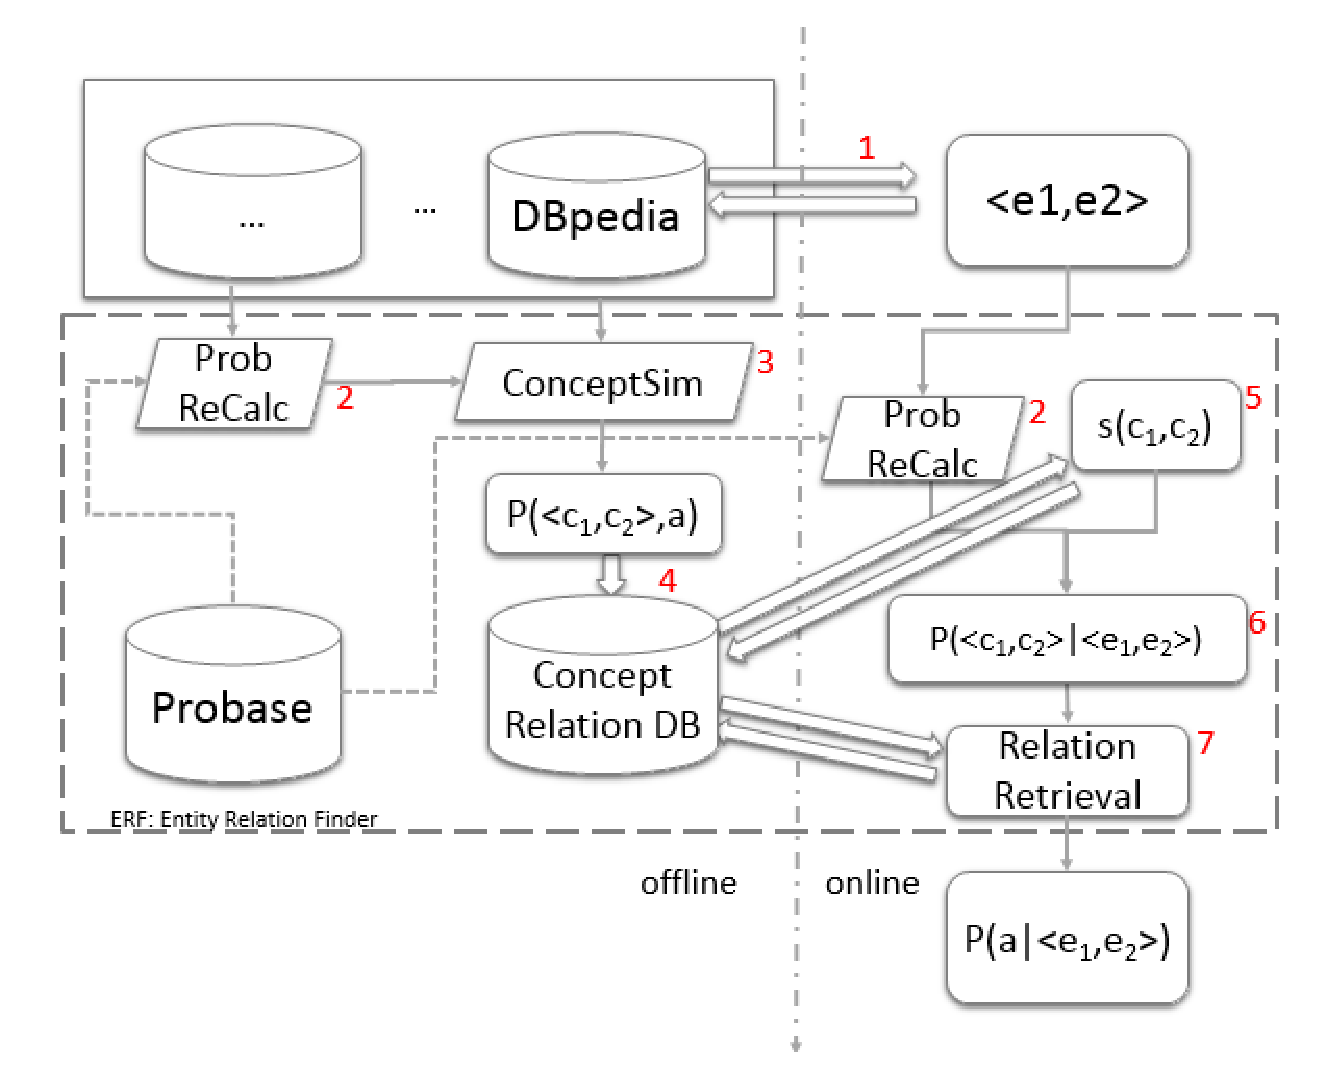
\epsfig{file=resources/framework.eps,width=\columnwidth}
\caption{Framework }
\end{figure}


In the offline component, we estimate all the probabilities that are independent of a specific entities pairs, including $s(c_1,c_2)$ and $P((c_{1},c_{2})|a)$ for each $a\in A$.
We leverage the DBpedia triples to learn these probabilities.
The online component accepts an entity pair $<e_1, e_2>$ as the query and calculate $ P(a| <e_1,e_2> )$ for each candidate attribute in $A$ by Eq.~\ref{eq:target_expand_all}. We return the the attribute owning the maximal score as the explanation for the relationship between the entity pair.

\yh{give a paragraph to explain how we do when no direct explanation can be found?}

\paragraph{Paper Orgnization}
The rest of the paper is organized as follows, Section~\ref{sec:conceptualization} describe how to derive $P(c|e)$ leveraging the \xch{basicness} of concept, Section~\ref{sec:fafa} is devoted to the offline calculation of $JD(c_1,c_2)$ and $P((c_{1},c_{2})|a)$.


\subsection{Notation Table}
\begin{table}[htbp]
  \centering
  \caption{Notation Table}
    \begin{tabular}{rr}
    \toprule
    notation & meaning \\
    \midrule
    $a$     & attribute \\
    $e_i$  & entity \\
    $c_i$  & concept \\
    $n(\cdot)$  & CountOf \\
    $c_h$  & head concept \\
    $c_l$  & long concept \\
    \bottomrule
    \end{tabular}%
  \label{tab:notation}%
\end{table}%


%First,we do conceptualization.
%
%Next,Judge whether the 2 entities are conceptually same
%
%Then, there are 2 cases of the CanBeExplained function:
%
%\begin{itemize}
%\item Explain 2 conceptually similar entity
%
%\begin{table}[htbp]
%  \centering
%  \caption{conceptually similar entity}
%    \begin{tabular}{rr}
%    \toprule
%    entity & concept \\
%    \midrule
%    Steve jobs & Person \\
%    Bill Gates & Person \\
%    \bottomrule
%    \end{tabular}%
%  \label{tab:addlabel}%
%\end{table}%
%
%
%\item Explain 2 conceptually different entity
%% Table generated by Excel2LaTeX from sheet 'Sheet1'
%\begin{table}[htbp]
%  \centering
%  \caption{Add caption}
%    \begin{tabular}{rr}
%    \toprule
%    entity & concept \\
%    \midrule
%    Mona Lisa & Painting \\
%    Renaissance & Period \\
%    \bottomrule
%    \end{tabular}%
%  \label{tab:addlabel}%
%\end{table}%
%
%Note that the concept here are not unique.
%
%\end{itemize}
%
%
%Last, We rank all the explanations in each step.
%
%
%
